\documentclass[11pt]{article}
\usepackage[margin=1in]{geometry}
\usepackage{amsmath,amssymb,amsthm,mathtools}
\usepackage{graphicx,booktabs,xcolor}
\usepackage[colorlinks=true,linkcolor=blue!50!black,citecolor=blue!50!black,urlcolor=blue!50!black]{hyperref}
\graphicspath{{figs/}}

\newtheorem{theorem}{Theorem}[section]
\newtheorem{proposition}[theorem]{Proposition}
\theoremstyle{definition}
\newtheorem{definition}[theorem]{Definition}
\newtheorem{example}[theorem]{Example}
\theoremstyle{remark}
\newtheorem*{intuition}{Intuition}
\newtheorem*{exercise}{Check yourself}

\newcommand{\N}{\mathcal N}
\newcommand{\E}{\mathbb E}
\newcommand{\R}{\mathbb R}
\newcommand{\tr}{\operatorname{tr}}
\newcommand{\KL}{\mathrm{KL}}
\newcommand{\nb}{\texttt{01\_feldman\_hajek.ipynb}}

\title{Learning notes: Gaussian measures, equivalence, and the aquifer prior}
\author{Raj Mahat}
\date{Started 14 October 2026 \quad--\quad compiled \today}

\begin{document}
\maketitle

\noindent These notes go slowly through the mathematics behind the \texttt{gw\_demarcation} experiment.
Every figure is produced by a Jupyter notebook in this folder, so each statement can be checked by
running code. Chapter~1 pairs with \nb.

\tableofcontents

%======================================================================
\section{Feldman--H\'ajek: when are two Gaussian priors ``the same kind of thing''?}
%======================================================================

\paragraph{Why we care.}
In the project we have a reference prior $P$, the stationary SPDE $(\kappa_0^2-\Delta)u=\xi$, and
alternatives $Q$ in which wells, a leakage bump, or a conductivity lens are added. Whenever we
compare, learn, or sample, we implicitly use the density ratio $dQ/dP$: likelihood ratios, KL
divergences, MCMC acceptance ratios, ``correct the reference by a few directions''. On a fixed
mesh this ratio always exists. The question is whether it \emph{survives mesh refinement}. If it
does not, every one of those quantities blows up as the mesh gets finer, and no fixed-size correction
can repair the reference. The Feldman--H\'ajek theorem tells us exactly when this happens.

\begin{intuition}
Two Gaussian measures are equivalent if and only if a single, infinitely resolved sample cannot tell
you which of the two produced it. If one perfect sample \emph{can} tell them apart, they are
mutually singular.
\end{intuition}

Everything below builds toward this sentence and then checks it with numbers.

%----------------------------------------------------------------------
\subsection{Equivalent and singular measures}

\begin{definition}
Let $P,Q$ be probability measures on the same space.
\begin{itemize}
\item $Q$ is \emph{absolutely continuous} w.r.t.\ $P$ ($Q\ll P$) if $P(E)=0\Rightarrow Q(E)=0$ for every event $E$.
\item $P$ and $Q$ are \emph{equivalent} ($P\sim Q$) if $Q\ll P$ and $P\ll Q$: they have the same impossible events.
\item $P$ and $Q$ are \emph{mutually singular} ($P\perp Q$) if there is an event $E$ with $P(E)=1$ and $Q(E)=0$: they live on disjoint sets.
\end{itemize}
\end{definition}

By the Radon--Nikodym theorem, $Q\ll P$ exactly when there is a density $\frac{dQ}{dP}$ with
$Q(E)=\int_E \frac{dQ}{dP}\,dP$. For equivalent measures the density is finite and positive
($P$-almost surely).

\paragraph{Finite dimensions: equivalence is the default.}
$P=\N(0,1)$ and $Q=\N(0,1.5^2)$ have
\[
\frac{dQ}{dP}(x)=\frac{1}{1.5}\exp\!\Big(\frac{x^2}{2}\big(1-1.5^{-2}\big)\Big),
\]
which is finite and positive for every $x$ (Fig.~\ref{fig:finite}b). The only way two Gaussians on
$\R^n$ can be singular is if one is degenerate and lives on a lower-dimensional subspace
(Fig.~\ref{fig:finite}c). In general, two \emph{non-degenerate} Gaussians on $\R^n$ are always
equivalent, however different their means and covariances are.

\begin{figure}[ht]\centering
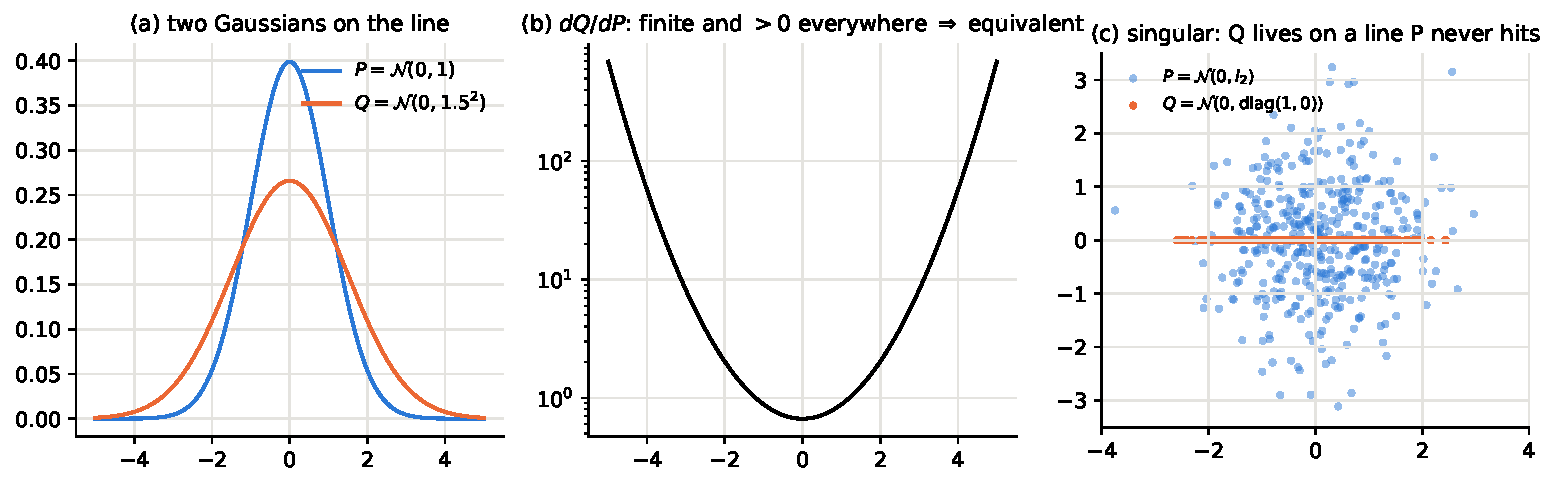
\includegraphics[width=\linewidth]{fh01_finite_dim.pdf}
\caption{Finite dimensions. (a,b) Two non-degenerate Gaussians are equivalent: the density ratio is
finite and positive everywhere. (c) A degenerate Gaussian sits on a line, which has probability 0
under $\N(0,I_2)$, so the two measures are singular.}
\label{fig:finite}
\end{figure}

So singularity is an \emph{infinite-dimensional} phenomenon. On a function space, as on an
ever-finer mesh, it arises without any degeneracy.

%----------------------------------------------------------------------
\subsection{Infinitely many independent coordinates}

Take $x=(x_1,x_2,\dots)$ with
\[
P=\N(0,I),\qquad Q=\N\big(0,\operatorname{diag}(1+t_j)\big),\qquad t_j>-1 .
\]
$t_j$ is the relative change of variance in coordinate $j$. Restricted to the first $n$
coordinates, both measures are non-degenerate Gaussians and the log density ratio of one sample is
a sum of independent terms:
\begin{equation}\label{eq:llr}
\ell_n(x)=\log\frac{dQ}{dP}(x)=\sum_{j=1}^n\Big[-\tfrac12\log(1+t_j)+\tfrac12\,\frac{t_j}{1+t_j}\,x_j^2\Big].
\end{equation}

\paragraph{Mean and spread of the one-sample statistic.}
Using $\E x_j^2=1$ under $P$, $\E x_j^2=1+t_j$ under $Q$ and $\operatorname{Var}(x_j^2)=2(\E x_j^2)^2$:
\begin{align*}
\E_Q\,\ell_n &= \tfrac12\sum_j\big(t_j-\log(1+t_j)\big)=\KL(Q\|P)\approx \tfrac14\sum_j t_j^2,\\
\E_P\,\ell_n &= -\tfrac12\sum_j\Big(\log(1+t_j)-\tfrac{t_j}{1+t_j}\Big)=-\KL(P\|Q)\approx -\tfrac14\sum_j t_j^2,\\
\operatorname{Var}_P\ell_n &= \tfrac12\sum_j\Big(\tfrac{t_j}{1+t_j}\Big)^2\approx \tfrac12\sum_j t_j^2 ,
\end{align*}
where $\approx$ is for small $t_j$. The two histograms of $\ell_n$ (one for samples from $P$, one
for samples from $Q$) are therefore separated by about $\tfrac12\sum t_j^2$, while each has width
about $\sqrt{\tfrac12\sum t_j^2}$. Their separation in units of width is
\[
\frac{\text{gap}}{\text{width}}\approx\sqrt{\tfrac12\textstyle\sum_{j\le n} t_j^2}\;.
\]

\begin{proposition}[Diagonal Feldman--H\'ajek]
If $\sum_j t_j^2=\infty$, one sample identifies the measure with certainty as $n\to\infty$, so
$P\perp Q$. If $\sum_j t_j^2<\infty$, the histograms keep a fixed overlap and $P\sim Q$.
\end{proposition}

The rigorous version is \textbf{Kakutani's theorem} (1948). Products of equivalent measures
$\bigotimes P_j$ and $\bigotimes Q_j$ are equivalent iff the product of Hellinger affinities
$\prod_j\rho_j$ is positive, and otherwise singular. For one Gaussian coordinate
\[
\rho_j=\int\sqrt{p_j q_j}\,dx=\Big(\frac{2\sqrt{1+t_j}}{2+t_j}\Big)^{1/2},
\qquad -\log\rho_j=\frac{t_j^2}{16}+O(t_j^3),
\]
so $\prod\rho_j>0\iff\sum t_j^2<\infty$. Note the \emph{dichotomy}: there is no in-between.
Gaussian measures are either equivalent or singular.

\paragraph{i.i.d.\ case.} With $t_j=0.2$ for all $j$, every coordinate is a harmless 20\% change,
yet $\sum t_j^2=\infty$. Fig.~\ref{fig:iid} shows the best one-sample test, ``say $Q$ iff
$\ell_n>0$'', going from coin-flipping at $n=1$ to never erring at $n=10^4$. The reason is the law
of large numbers: $\frac1n\sum x_j^2\to1$ under $P$ and $\to1.2$ under $Q$. These two events are
disjoint and carry probability one under their own measure.

\begin{figure}[ht]\centering
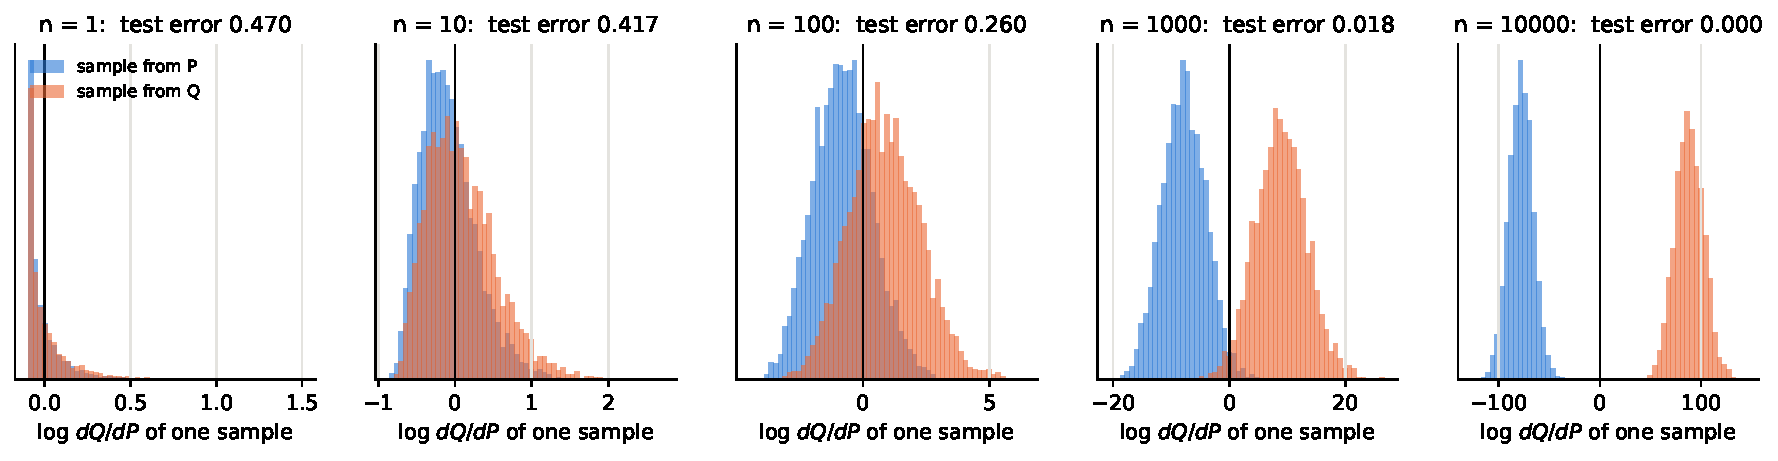
\includegraphics[width=\linewidth]{fh02_iid_separation.pdf}
\caption{$t_j=0.2$ in every coordinate. Histograms of the one-sample log likelihood ratio
\eqref{eq:llr} under $P$ (blue) and $Q$ (orange). The title gives the error of the best test. As
the number of coordinates grows the histograms separate completely: singular.}
\label{fig:iid}
\end{figure}

\paragraph{Decaying perturbations.} Fig.~\ref{fig:decay} compares three sequences:
$t_j=0.2$ ($\sum t_j^2=\infty$, fast), $t_j=j^{-1/4}$ ($\sum t_j^2=\sum j^{-1/2}=\infty$, slow), and
$t_j=1/j$ ($\sum t_j^2=\pi^2/6$). For $t_j=1/j$ the affinity, the test error and the histograms all
\emph{freeze} as $n$ grows: extra coordinates bring no new evidence. That is what equivalence looks
like.

\begin{figure}[ht]\centering
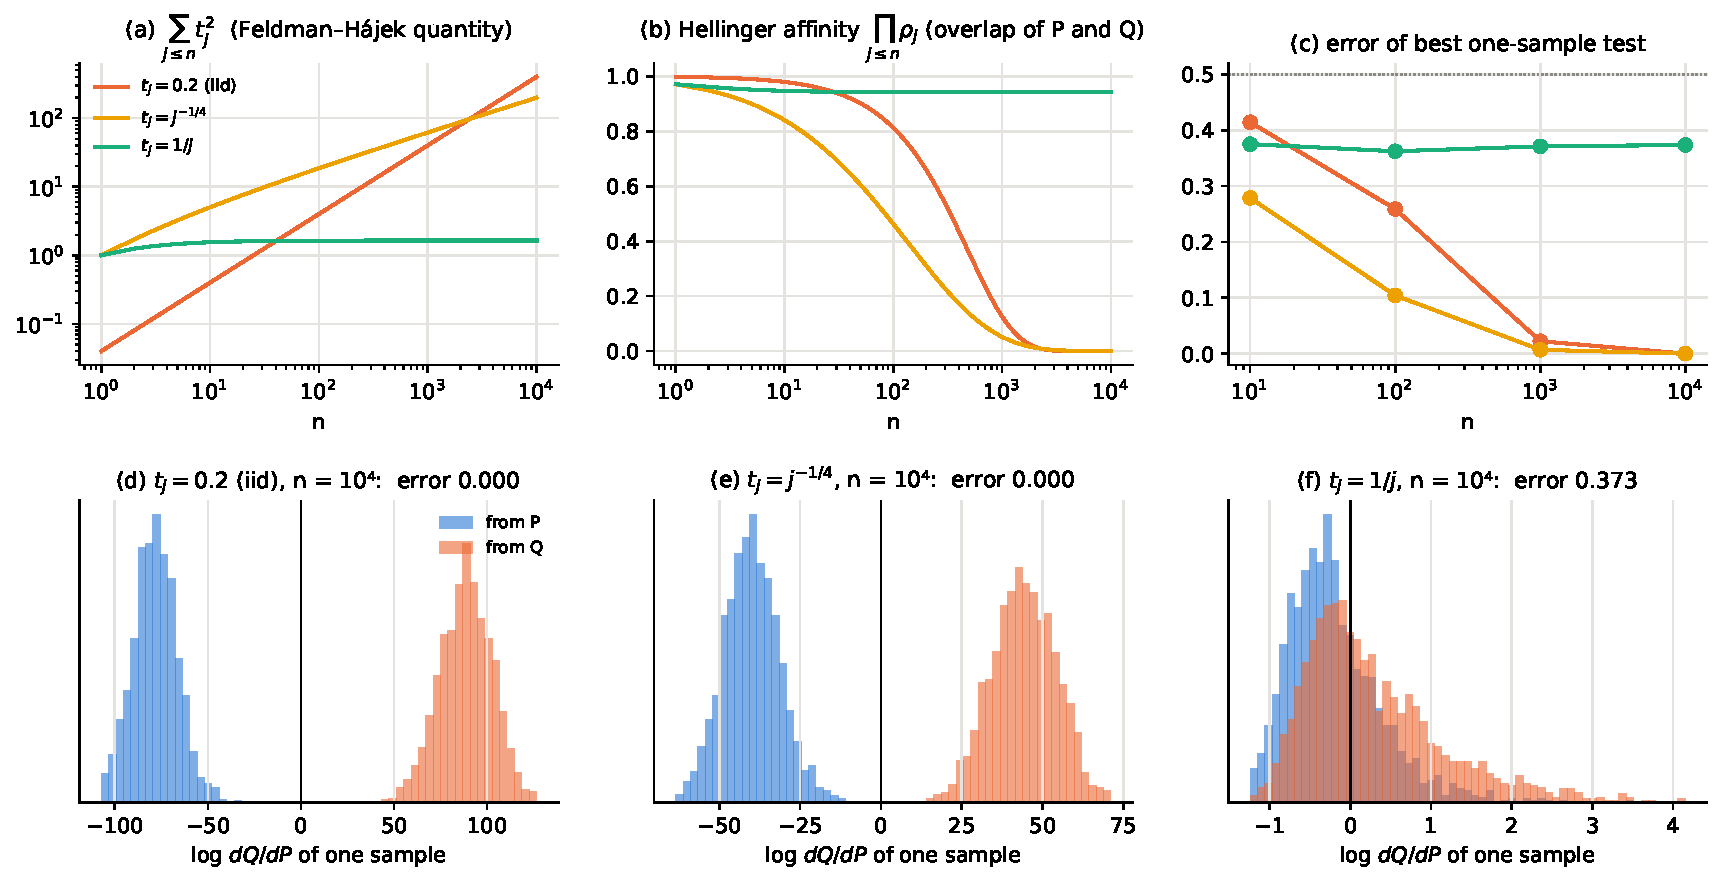
\includegraphics[width=\linewidth]{fh03_decay_kakutani.pdf}
\caption{(a) The Feldman--H\'ajek quantity $\sum_{j\le n}t_j^2$. (b) The overlap of $P$ and $Q$
(Hellinger affinity). (c) The best one-sample test error. (d--f) Histograms at $n=10^4$. Only
$t_j=1/j$, with a finite sum, keeps a permanent overlap.}
\label{fig:decay}
\end{figure}

\subsection{Mean shifts and the Cameron--Martin space}

So far $P$ and $Q$ had the same mean and different variances. Now keep the covariance and move the
mean:
\[
P=\N(0,I_n),\qquad Q=\N(m,I_n),\qquad m=(m_1,\dots,m_n).
\]
Every $x_j$ still has variance 1; under $Q$ it is centred at $m_j$ instead of 0.

\paragraph{The one-sample statistic.}
Writing out the two Gaussian densities, the $x_j^2$ terms cancel and
\[
\ell_n(x)=\log\frac{dQ}{dP}(x)=\sum_{j=1}^n\Big(m_jx_j-\tfrac12 m_j^2\Big)=\langle m,x\rangle-\tfrac12\|m\|^2 .
\]
This is a \emph{matched filter}: project the sample onto the direction $m$ and compare with the
midpoint. It is linear in $x$, so it is exactly Gaussian:
\begin{align*}
x\sim P:&\quad \langle m,x\rangle\sim\N(0,\|m\|^2) &&\Rightarrow\quad \ell_n\sim\N\big(-\tfrac12\|m\|^2,\ \|m\|^2\big),\\
x\sim Q:&\quad \langle m,x\rangle=\|m\|^2+\langle m,z\rangle &&\Rightarrow\quad \ell_n\sim\N\big(+\tfrac12\|m\|^2,\ \|m\|^2\big).
\end{align*}
The two histograms are separated by $\|m\|^2$ and each has width $\|m\|$. Gap over width is $\|m\|$,
and the best test (say $Q$ iff $\ell_n>0$) has error $\Phi(-\|m\|/2)$.

\paragraph{Geometric picture.} Along the direction $m/\|m\|$ the noise has standard deviation 1
(white noise has the same spread in every direction), while the signal has length $\|m\|$. The
signal-to-noise ratio is $\|m\|$. Each coordinate contributes $m_j^2$ to $\|m\|^2$, so $m_j^2$ is
the evidence coordinate $j$ supplies, just as $t_j^2$ was for variances.
\[
P\sim Q\iff \|m\|^2=\sum_j m_j^2<\infty .
\]

\paragraph{Examples (Fig.~\ref{fig:mean}).}
\begin{itemize}
\item $m_j=1/j$: $\|m\|^2\to\pi^2/6\approx1.64$, $\|m\|\approx1.28$. The error freezes at
$\Phi(-0.64)\approx0.26$ however many coordinates are added: \textbf{equivalent}.
\item $m_j=1/\sqrt j$: $\|m\|^2=\sum 1/j\approx\log n+0.58\to\infty$. The error decays to 0, but only
logarithmically: at $n=10^4$, $\|m\|\approx3.1$ and the error is still $\approx0.06$. Even so, it is
\textbf{singular}. Each individual shift $m_j\to0$, but not fast enough.
\end{itemize}

\paragraph{When the coordinates are not white: the Cameron--Martin space.}
For a general prior $P=\N(0,C)$ with eigenpairs $(\lambda_j,\phi_j)$, coordinate $j$ has noise standard
deviation $\sqrt{\lambda_j}$. A shift $m_j=\langle m,\phi_j\rangle$ must be measured in units of that
noise: whitening gives $\tilde m_j=m_j/\sqrt{\lambda_j}$, and
\[
P\sim Q\iff \sum_j\frac{m_j^2}{\lambda_j}=\|C^{-1/2}m\|^2<\infty
\iff m\in\mathcal H_P:=C^{1/2}H .
\]
$\mathcal H_P$ is the \emph{Cameron--Martin space} of $P$. Because $\lambda_j\to0$ quickly for a smooth
prior, fine-scale coordinates are expensive. A shift that has any appreciable fine-scale content is
fatal, because the prior has almost no noise there to hide it in.

\paragraph{For our SPDE prior.} $(\kappa^2-\Delta)u=\xi$ has $\lambda_j=(\kappa^2+\mu_j)^{-2}$, where the
$\mu_j$ are the Dirichlet Laplacian eigenvalues. Then
\[
\|C^{-1/2}m\|^2=\sum_j(\kappa^2+\mu_j)^2m_j^2=\|(\kappa^2-\Delta)m\|_{L^2}^2 ,
\]
so $\mathcal H_P=\{m:(\kappa^2-\Delta)m\in L^2,\ m=0\text{ on }\partial\Omega\}$, the Sobolev space
$H^2$ with boundary conditions. Two consequences follow.
\begin{itemize}
\item \textbf{A typical sample is \emph{not} in its own Cameron--Martin space.} For a sample $u$,
$(\kappa^2-\Delta)u=\xi$ is white noise, and $\|\xi\|_{L^2}^2=\sum\xi_j^2=\infty$. So shifting the prior by
one of its own typical draws gives a singular measure. The Cameron--Martin space is much smoother
than the samples: it has probability zero under $P$.
\item \textbf{Deterministic wells.} A known pumping $q=\xi+a\,g$ shifts the mean by $m=a(\kappa^2-\Delta)^{-1}g$.
Then $\|C^{-1/2}m\|=|a|\,\|g\|_{L^2}$, so the shifted prior is equivalent iff $g\in L^2$. A smooth or
extended well is fine. A \emph{point} well $g=\delta_{x_0}$ is not in $L^2$ (in any dimension), so its
mean shift is singular. On a mesh, $\delta$ becomes a spike of height $1/h^d$ at one node, and
$\|g\|^2\approx h^{-d}\to\infty$.
\end{itemize}
The \emph{random} wells of the project ($a\sim\N(0,c)$) give the covariance version of the same
condition. In whitened coordinates the added eigenvalue is $t=c\,\|g\|_{L^2}^2$, finite iff
$g\in L^2$ (\S\ref{sec:aquifer}: $t=c\,h\,g^\top g$).

\begin{figure}[ht]\centering
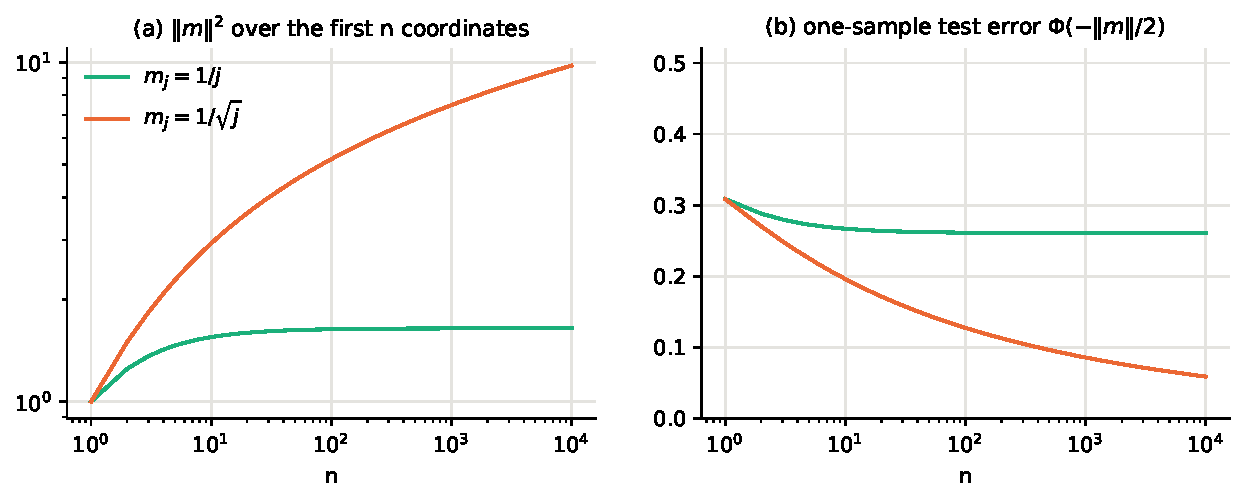
\includegraphics[width=.8\linewidth]{fh04_mean_shift.pdf}
\caption{Mean shifts. $m_j=1/j$ has finite $\|m\|$, so the measures are equivalent. $m_j=1/\sqrt j$
has infinite $\|m\|$, so they are singular.}
\label{fig:mean}
\end{figure}

%----------------------------------------------------------------------
\subsection{The Feldman--H\'ajek theorem}

Remove the diagonal assumption. Let $H$ be a separable Hilbert space ($L^2(\Omega)$ for us), and
$P=\N(m_0,C_0)$, $Q=\N(m_1,C_1)$ Gaussian measures with injective trace-class covariances.

\begin{theorem}[Feldman 1958, H\'ajek 1958]\label{thm:fh}
$P$ and $Q$ are either equivalent or mutually singular. They are equivalent if and only if
\begin{enumerate}
\item[(i)] $C_0^{1/2}H=C_1^{1/2}H$ (same Cameron--Martin space);
\item[(ii)] $m_1-m_0\in C_0^{1/2}H$;
\item[(iii)] $T:=C_0^{-1/2}C_1C_0^{-1/2}-I$ is a \emph{Hilbert--Schmidt} operator, i.e.\
$\|T\|_{HS}^2=\sum_j t_j^2<\infty$, where $t_j$ are the eigenvalues of $T$.
\end{enumerate}
\end{theorem}

\noindent See Da Prato \& Zabczyk (2014, Thm.~2.25) or Bogachev (1998, Thm.~2.7.2).

\paragraph{How to read it: whitening.}
Let $z=C_0^{-1/2}(u-m_0)$. Under $P$, $z$ is white noise, $\N(0,I)$. Under $Q$ (taking $m_1=m_0$),
$z\sim\N(0,I+T)$. In the eigenbasis of $T$ this is exactly the diagonal problem of the previous
subsection, with the $t_j$ now the eigenvalues of $T$. Condition (iii) is $\sum t_j^2<\infty$.
Condition (ii) is $\sum m_j^2<\infty$ in whitened coordinates. Condition (i) is the technical
requirement that $T$ is well defined and $I+T$ is invertible, so no $t_j$ reaches $-1$.

\paragraph{KL divergence.} When $P\sim Q$ (zero means),
\begin{equation}\label{eq:kl}
\KL(Q\|P)=\tfrac12\sum_j\big(t_j-\log(1+t_j)\big)=\tfrac12\big(\tr T-\log\det(I+T)\big),
\end{equation}
which is finite exactly when $\sum t_j^2<\infty$, since $t-\log(1+t)\approx t^2/2$. If
$P\perp Q$, then $\KL=\infty$.

\paragraph{The mesh-refinement test.}
On an $N$-node mesh everything is finite. Compute the $N\times N$ matrix $T_N$ and watch
$\|T_N\|_F$ and $\KL_N$ as $N$ grows. A plateau means $P\sim Q$. Growth without bound means $P\perp Q$.
This is the diagnostic used in the main project (figures F1, F2).

%----------------------------------------------------------------------
\subsection{Random functions: range versus amplitude}\label{sec:range}

Take the 1D version of the reference prior on $[0,1]$ with $u(0)=u(1)=0$:
\[
(\kappa^2-\partial_x^2)\,u=\tau\,\xi .
\]
The sine functions $\phi_j(x)=\sqrt2\sin(j\pi x)$ are eigenfunctions of $-\partial_x^2$ with
$\lambda_j=(j\pi)^2$. Hence
\[
u=\sum_j c_j\,\phi_j,\qquad c_j\sim\N\Big(0,\frac{\tau^2}{(\kappa^2+\lambda_j)^2}\Big)\ \text{independent.}
\]
Two such priors are diagonal in the same basis, with $1+t_j=\mathrm{var}_Q(c_j)/\mathrm{var}_P(c_j)$.

\begin{itemize}
\item \textbf{Range change} $\kappa_0\to\kappa_1$ (with $\tau$ fixed):
$t_j=\big(\frac{\kappa_0^2+\lambda_j}{\kappa_1^2+\lambda_j}\big)^2-1\approx\frac{2(\kappa_0^2-\kappa_1^2)}{\pi^2j^2}$.
So $\sum t_j^2<\infty$: \textbf{equivalent}.
\item \textbf{Amplitude change} $\tau_0\to\tau_1$: $t_j=\tau_1^2/\tau_0^2-1$ for every $j$. This is the i.i.d.\ case: \textbf{singular}.
\end{itemize}

\begin{figure}[ht]\centering
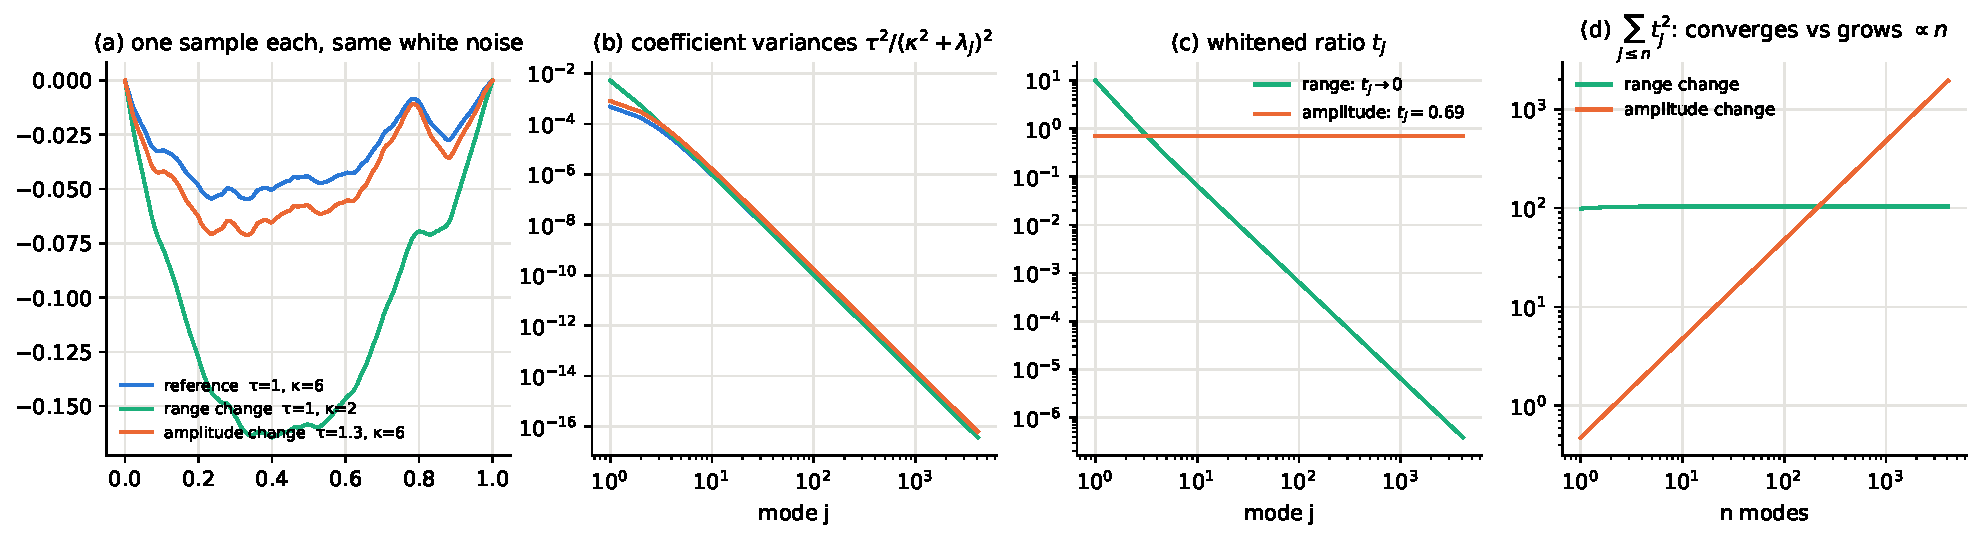
\includegraphics[width=\linewidth]{fh05_range_vs_amplitude.pdf}
\caption{(a) One sample from the reference ($\tau=1,\kappa=6$), a range change ($\kappa=2$) and an
amplitude change ($\tau=1.3$), all driven by the same white noise. (b) Coefficient variances: the
range change merges with the reference at high modes, while the amplitude change stays parallel
forever. (c) $t_j$. (d) $\sum t_j^2$ converges (to $\approx104$, dominated by the first mode) for the
range change and grows linearly for the amplitude change.}
\label{fig:range}
\end{figure}

\paragraph{The surprise (Fig.~\ref{fig:range}a).}
The range change looks the most different to the eye, with bigger and smoother excursions, yet it is
the \emph{equivalent} one. The amplitude change looks almost like the reference, yet it is
\emph{singular}. Equivalence is decided by the \textbf{fine scales}, because there are infinitely
many of them. A large-scale difference lives in finitely many modes, however dramatic it looks, and a
single sample can never confirm it with certainty.

\paragraph{Higher dimensions.} In $d$ dimensions the number of modes with $\lambda\le\Lambda$ grows
like $\Lambda^{d/2}$, and for a range change $t\sim1/\lambda$. Then
$\sum t^2\sim\int^\infty\Lambda^{d/2-1}\Lambda^{-2}\,d\Lambda<\infty$ iff $d<4$. Range changes are
harmless in $d\le3$, which is Bolin \& Kirchner's Cor.~3.3.

\paragraph{The flip side: what one sample can teach you (microergodicity).}
Fit $(\tau,\kappa)$ by maximum likelihood to \emph{one} sample resolved to $N$ modes. The Fisher
information is
\[
I_\tau(N)=\frac{2N}{\tau^2}\to\infty,\qquad
I_\kappa(N)=\frac12\sum_{j\le N}\Big(\frac{4\kappa}{\kappa^2+\lambda_j}\Big)^2\to\text{const}<\infty .
\]
$\hat\tau$ becomes exact as the sample is refined, while $\hat\kappa$ never settles
(Fig.~\ref{fig:micro}). In the notebook the spread of $\hat\tau$ falls from $0.26$ to $0.01$
between $N=16$ and $4096$, while the spread of $\hat\kappa$ stays near $2.5$. This is the same fact
as before, seen from the other side: parameters that change the measure's class are learnable
from one sample, and parameters that keep it equivalent are not. $\tau$ (more precisely
$\sigma^2\kappa^{2\nu}$ in Mat\'ern form) is the \emph{microergodic} parameter (Zhang 2004).

\begin{figure}[ht]\centering
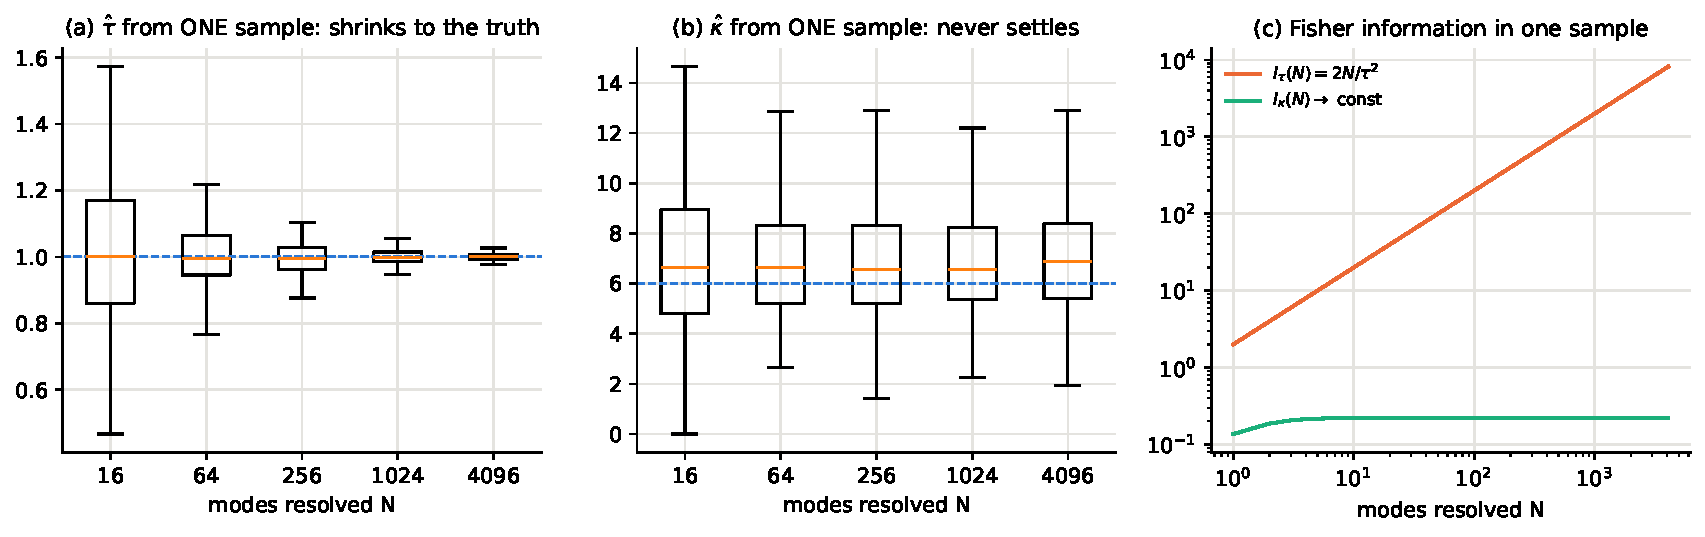
\includegraphics[width=\linewidth]{fh06_microergodic.pdf}
\caption{Maximum-likelihood estimates from a single sample (300 replicates, truth $\tau=1,\kappa=6$).
(a) $\hat\tau$ converges as the resolution grows. (b) $\hat\kappa$ does not. (c) Fisher information:
unbounded for $\tau$, bounded for $\kappa$.}
\label{fig:micro}
\end{figure}

\paragraph{Link to the project.} Because $\kappa$ costs almost nothing in likelihood, it is the
knob a stationary fit turns to absorb unmodelled large-scale variance. With the wells present, M1
slid to $\hat\kappa\approx0$.

%----------------------------------------------------------------------
\subsection{Back to the aquifer, in one dimension}\label{sec:aquifer}

Discretize $-(Ku')'+\kappa^2(x)u=q$ on $N$ interior nodes with spacing $h=1/(N+1)$, with $K$ evaluated
at cell faces. This gives a tridiagonal $A$ with $Au=q$. With discrete white noise
$\xi_i\sim\N(0,1/h)$,
\[
\Sigma=h^{-1}A^{-1}A^{-\top},\qquad \text{precision } Q=h\,A^\top A .
\]
Choosing the square root $\Sigma_0^{1/2}=h^{-1/2}A_0^{-1}$ gives
\[
I+T=\Sigma_0^{-1/2}\Sigma_1\Sigma_0^{-\top/2}=B B^\top,\qquad B=A_0A_1^{-1},
\]
so the eigenvalues of $T$ are the squared singular values of $A_0A_1^{-1}$ minus one. The
reference is $K\equiv1$, $\kappa^2\equiv36$. The three truths are:

\begin{center}
\begin{tabular}{lll}
\toprule
truth & change & place in the equation \\
\midrule
well & $q=\xi+a\,g$, $a\sim\N(0,50)$, $g$ a smooth bump with $\int g^2=1$ & source \\
leakage & $\kappa^2(x)=36-30\,e^{-((x-0.75)/0.06)^2}$ & zeroth order \\
lens & $K(x)=e^{b(x)}$, $b\approx1$ on $[0.4,0.6]$ & principal part \\
\bottomrule
\end{tabular}
\end{center}

\begin{figure}[ht]\centering
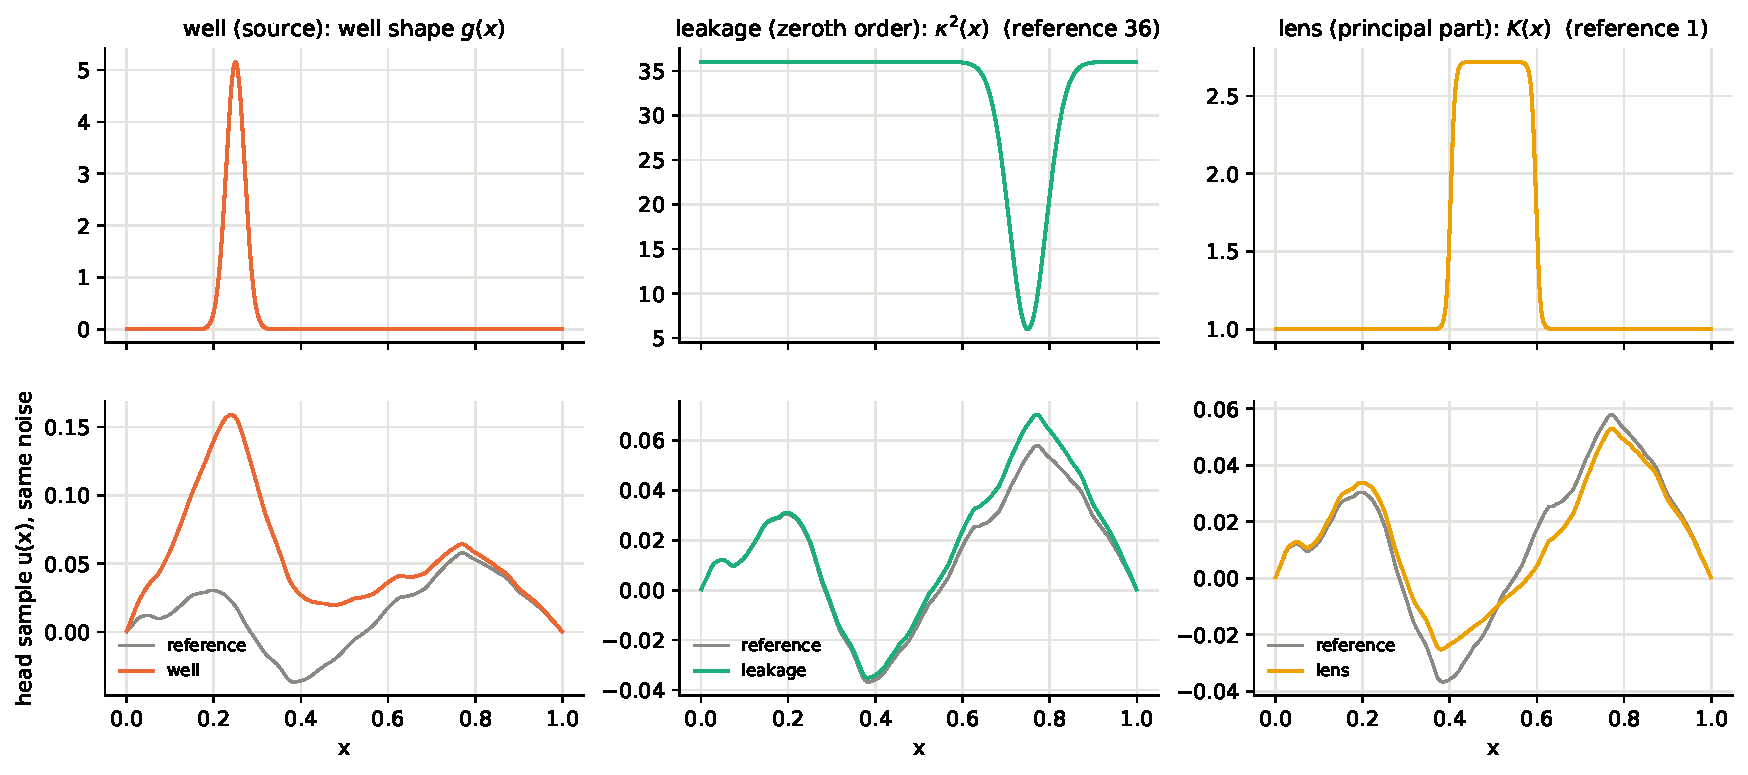
\includegraphics[width=\linewidth]{fh07_aquifer_1d_setup.pdf}
\caption{Top: the three departures. Bottom: one head sample under the reference (grey) and under
each truth (colour), all from the same white noise.}
\label{fig:aq-setup}
\end{figure}

\paragraph{What to expect.}
\begin{itemize}
\item The \textbf{well} adds the rank-one term $c\,A_0^{-1}gg^\top A_0^{-\top}$. In whitened
coordinates this is a single eigenvalue $t=c\,h\,g^\top g\approx c\int g^2=50$ and zeros elsewhere.
That is trivially Hilbert--Schmidt: equivalent.
\item The \textbf{leakage} change perturbs the operator by a bounded multiplication, $\delta\kappa^2$,
which is lower order than $-\partial_x^2$. Whitened, it behaves like $(\kappa^2-\partial_x^2)^{-1}$
times something bounded, so $t_j\sim1/\lambda_j$: Hilbert--Schmidt in $d\le3$. Equivalent.
\item The \textbf{lens} changes the highest-order term. At fine scales $A_1\approx-\partial_x K\partial_x$
and $A_0\approx-\partial_x^2$, so $BB^\top$ acts locally like multiplication by $K(x)^{-2}$, and
$T$ like multiplication by $K^{-2}-1$. A multiplication operator is not compact. A fixed
\emph{fraction} of all $N$ eigenvalues (the fraction of the domain covered by the lens) sits near
$e^{-2}-1\approx-0.86$, so $\|T\|_F^2\propto N$. Singular.
\end{itemize}

\begin{figure}[ht]\centering
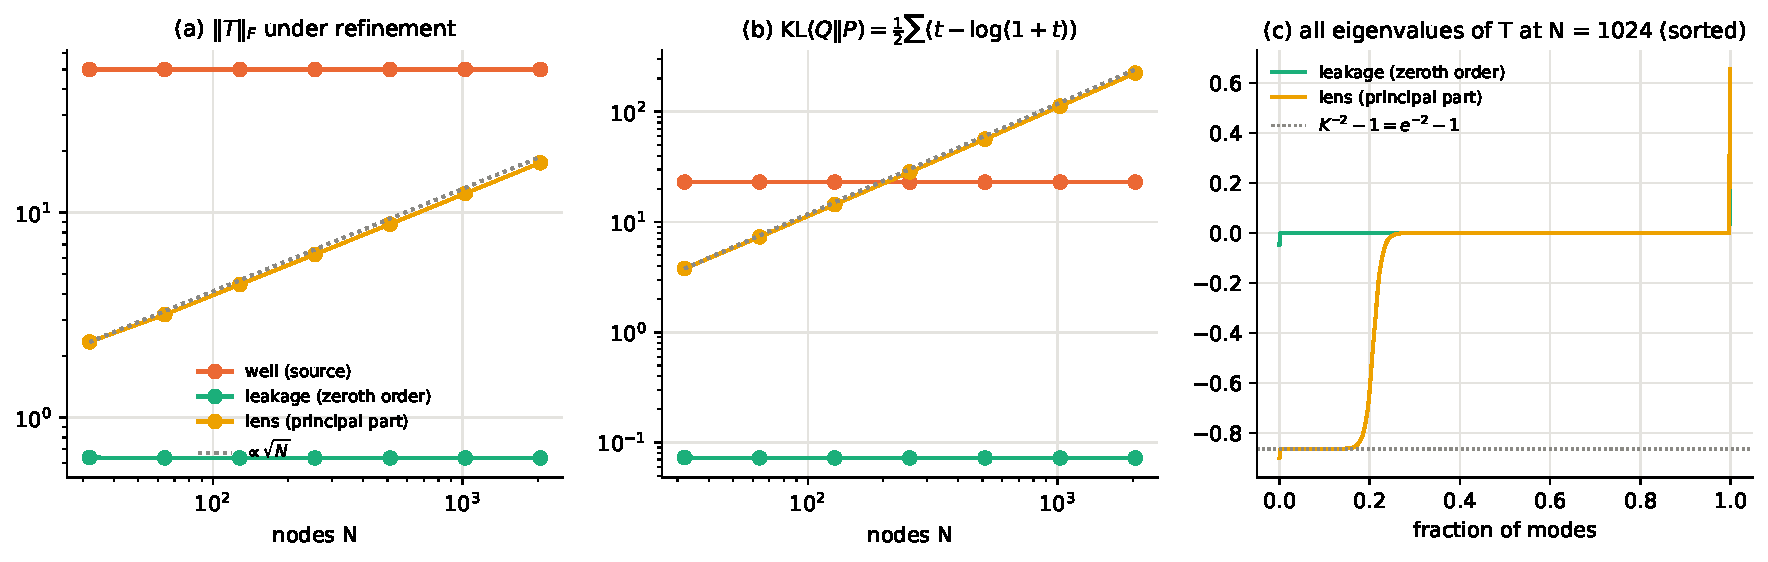
\includegraphics[width=\linewidth]{fh08_aquifer_refinement.pdf}
\caption{(a) $\|T\|_F$ and (b) $\KL$ under mesh refinement. The well and the leakage are flat; the
lens grows like $\sqrt N$ and $N$. (c) All eigenvalues of $T$ at $N=1024$: about 20\% of them sit
at the symbol value $K^{-2}-1$.}
\label{fig:aq-ref}
\end{figure}

\begin{center}
\begin{tabular}{rccc}
\toprule
$N$ & well & leakage & lens \\
\midrule
32 & 50.00 & 0.638 & 2.34 \\
128 & 50.00 & 0.635 & 4.46 \\
512 & 50.00 & 0.635 & 8.80 \\
2048 & 50.00 & 0.635 & 17.52 \\
\bottomrule
\end{tabular}

\smallskip
$\|T_N\|_F$ from the notebook. The lens grows by $\sqrt2$ per doubling of $N$.
\end{center}

\noindent In 2D, $N=n^2$, so $\|T\|_F\propto n$ and $\KL\propto n^2$, which is exactly what the
main project measured (F1). Note the scale. The well has a \emph{much larger} $\|T\|_F$ (50) than the
lens at any mesh shown here, yet it is the lens that is singular. As with the range change, what
matters is not the size of the departure but whether it reaches the fine scales.

\paragraph{The one-sample test, for heads.}
Repeat the experiment of Fig.~\ref{fig:iid} with real head fields, using
\[
\log\frac{d\mu_1}{d\mu_0}(u)=\log|A_1|-\log|A_0|-\tfrac h2\big(\|A_1u\|^2-\|A_0u\|^2\big),
\]
and a Woodbury form for the well. Fig.~\ref{fig:aq-test} shows the result. For the well and the
leakage the error of the best test does not change with $N$: a finer mesh gives no new evidence. For
the lens the error drops to zero. A finely resolved head field carries the lens's fingerprint in
every small-scale wiggle.

\begin{figure}[ht]\centering
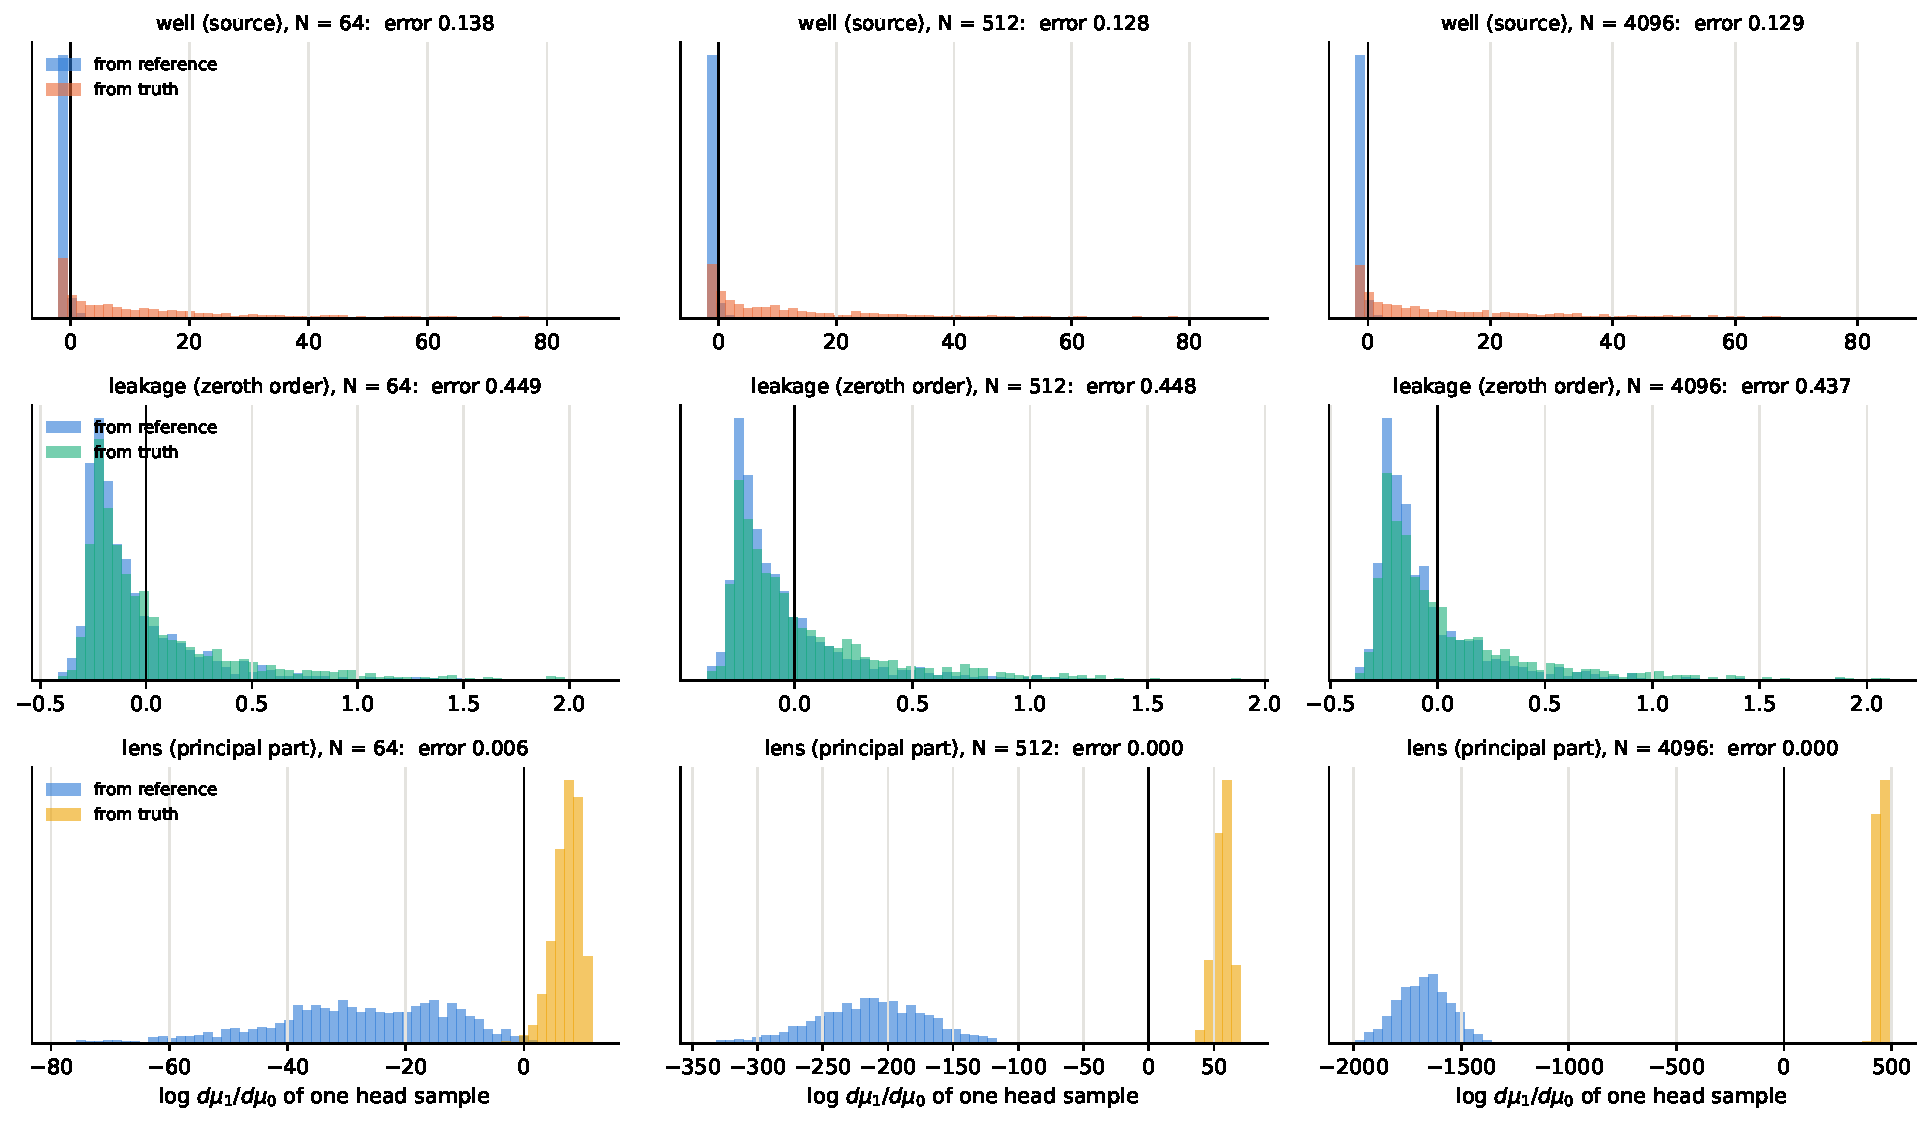
\includegraphics[width=\linewidth]{fh09_aquifer_one_sample_test.pdf}
\caption{One-sample log likelihood ratio, reference versus truth, at $N=64, 512, 4096$. The well
(error $\approx0.13$) and the leakage (error $\approx0.44$) are stable: equivalent. The lens error is
$0.006\to0.000$: singular.}
\label{fig:aq-test}
\end{figure}

%----------------------------------------------------------------------
\subsection{Take-aways}
\begin{enumerate}
\item Equivalence means the same null sets, which means a density $dQ/dP$ exists, which means one
perfect sample cannot tell the measures apart.
\item Diagonal case: equivalent iff $\sum t_j^2<\infty$ (variances) and $\sum m_j^2<\infty$ (means).
Feldman--H\'ajek is the same statement without a basis: $T$ is Hilbert--Schmidt and the mean
lies in the Cameron--Martin space.
\item The decision is made at the \textbf{fine scales}. Large-scale changes (range $\kappa$, wells,
leakage) are harmless however big they look. Changes that persist down to the smallest scales
(amplitude $\tau$, conductivity $K$) are fatal however small they look.
\item Practically: what a fine sample determines exactly ($\tau$, $K$) cannot be ``corrected'' with
finitely many directions, and what it never determines ($\kappa$) is a cheap knob a fit can slide
along.
\end{enumerate}

\begin{exercise}
\begin{enumerate}
\item Is $t_j=1/\sqrt j$ equivalent or singular? Compute $\sum t_j^2$.
\item A constant conductivity $K\equiv2$: equivalent or singular? (Hint: $-\nabla\cdot(2\nabla u)+\kappa^2u=\xi$ is
$2\big(\tfrac{\kappa^2}{2}-\Delta\big)u=\xi$. Which parameter of \S\ref{sec:range} changed?)
\item The well's source shape $g$ must be in $L^2$, so that its head response $(\kappa^2-\Delta)^{-1}g$ is in $H^2$. What happens to $t=c\,h\,g^\top g$ when $g$ becomes a delta at the grid scale ($g_i=1/h$ at one node)?
\end{enumerate}
\end{exercise}

\paragraph{Next chapter (planned).} Whitening and the operator $T$ in 2D; why the lens's $T$ is ``multiplication by
$K^{-2}-1$'' (symbols of differential operators); then how the finite-rank model M3 sees $T$ through
sample covariances (Marchenko--Pastur, BBP).

\section*{References}
\begin{itemize}\small
\item V.~I.~Bogachev, \emph{Gaussian Measures}, AMS, 1998 (Thm.~2.7.2).
\item G.~Da Prato, J.~Zabczyk, \emph{Stochastic Equations in Infinite Dimensions}, 2nd ed., CUP, 2014 (Thm.~2.25).
\item J.~Feldman, Equivalence and perpendicularity of Gaussian processes, \emph{Pacific J.\ Math.}\ 8 (1958).
\item J.~H\'ajek, On a property of normal distributions of any stochastic process, \emph{Czech.\ Math.\ J.}\ 8 (1958).
\item S.~Kakutani, On equivalence of infinite product measures, \emph{Ann.\ Math.}\ 49 (1948).
\item H.~Zhang, Inconsistent estimation and asymptotically equal interpolations in model-based geostatistics, \emph{JASA} 99 (2004).
\item D.~Bolin, K.~Kirchner, Equivalence of measures and asymptotically optimal linear prediction for Gaussian random fields with fractional-order covariance operators, \emph{Bernoulli} 29(2) (2023).
\end{itemize}

\end{document}
